\chapter{Lec 16 - A 1.5-Approximation Algorithm for Metric TSP}

\section{Christofides' algorithm}
The \textit{APPROX\_METRIC\_TSP} algorithm has a 2-approximation factor because the full Preorder chain of $T^*$ uses every edge of $T^*$ twice. We'll try to improve on this by constructing a tour that traverses MST edges \textbf{only once}.\newline\newline
\textbf{Definition:} A path (or cycle) is \textbf{Eulerian} if it visits every edge of the graph exactly once.\newline\newline
\textbf{Definition}: A connected graph is Eulerian if it exists an Eulerian cycle.\newline\newline
If the MST was Eulerian (cannot be), we would have a 1-approximation algorithm. Our idea is to build a \textit{cheap} Eulerian cycle in the MST.\newline\newline
\textbf{Theorem:} A connected graph is Eulerian $\iff$ every vertex has even degree \footnote{if i want to traverse every edge exactly once, i must have a \textit{way out} from every vertex}.\newline\newline
So, let's handle the \textbf{odd degree} vertices of the MST explicitly.\newline\newline
\textbf{Property:} In any (finite) graph the number of vertices of odd degree is even.\newline\newline
\textbf{Proof:} The proof comes from the following equality:
\[\sum_{v \in V}deg(v) = 2m\]
Note that we can split the summation in two parts:
\[\sum_{u \in even} deg(u) + \sum_{w \in odd}deg(w) = 2m\]
Since the result must be even, $\sum_{w \in odd}deg(w)$ must be even. But this happens only if the number of odd degree vertices is even.\newline\newline
\textbf{Idea:} Augment the initial MST $T^*$ with a minimum-weight \textbf{perfect matching} between the vertices that have odd degree in the MST (perfect means that it includes all such vertices).\newline\newline
For example, let's consider the following MST $T^*$:\newline\newline
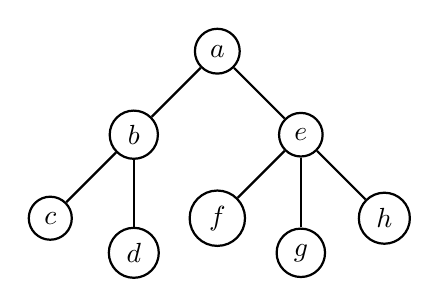
\begin{tikzpicture}[node distance={15mm}, thick, main/.style = {draw, circle}] 
            \node[main] (a) {$a$}; 
            \node[main] (b) [below left of=a] {$b$}; 
            \node[main] (e) [below right of=a] {$e$}; 
            \node[main] (c) [below left of=b] {$c$}; 
            \node[main] (d) [below of=b] {$d$};
            \node[main] (f) [below left of=e] {$f$};
            \node[main] (g) [below of=e] {$g$};
            \node[main] (h) [below right of=e] {$h$};

            \draw (a) -- (b); 
            \draw (a) -- (e); 
            \draw (b) -- (c);
            \draw (b) -- (d);
            \draw (e) -- (f);
            \draw (e) -- (g);
            \draw (e) -- (h);
\end{tikzpicture}\newline\newline
In this example the odd-degree vertices are $b, c, d, f, g, h$. If we augment $T^*$ with a minimum-weight perfect matching, it becomes as follows \footnote{Note that it's important that the odd-degree vertices are even, because in this case a perfect matching always exists.}:\newline\newline
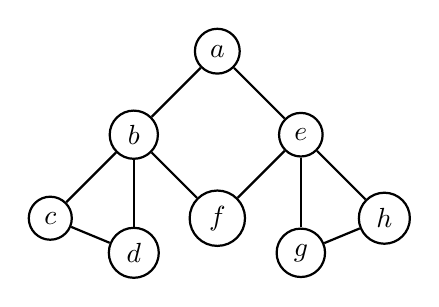
\begin{tikzpicture}[node distance={15mm}, thick, main/.style = {draw, circle}] 
            \node[main] (a) {$a$}; 
            \node[main] (b) [below left of=a] {$b$}; 
            \node[main] (e) [below right of=a] {$e$}; 
            \node[main] (c) [below left of=b] {$c$}; 
            \node[main] (d) [below of=b] {$d$};
            \node[main] (f) [below left of=e] {$f$};
            \node[main] (g) [below of=e] {$g$};
            \node[main] (h) [below right of=e] {$h$};

            \draw (a) -- (b); 
            \draw (a) -- (e); 
            \draw (b) -- (c);
            \draw (b) -- (d);
            \draw (e) -- (f);
            \draw (e) -- (g);
            \draw (e) -- (h);
            \draw (c) -- (d);
            \draw (b) -- (f);
            \draw (g) -- (h);
\end{tikzpicture}\newline\newline
The resulting graph has only even-degree vertices, that is, Eulerian graph. Now that we have an Eulerian graph, we can approximate a Metric TSP tour by finding an Eulerian cycle in this graph adding shortcuts when needed (as we did with \textit{APPROX\_METRIC\_TSP}).\newline\newline
\begin{algorithm}
\caption{Christofides' algorithm}\label{Christofides}
    \begin{algorithmic}[1]
    \Procedure{Christofides($G$)}{}
        \State $T^* = Prim(G, r) \quad //T^*=(V, E^*)$
        \State $D =$ set of vertices of $T^*$ with odd degree
        \State $M^* = $ a min-weight perfect matching on the graph iduced by $D \quad \text{// can be done in poly-time}$ 
        \State $G^* = (V, E^*) \cup M^* \quad \text{// this is an Eulerian graph}$

        \State $E= $ an Eulerian cycle on $G^*$
        \State \textbf{return} the cycle that visits all the vertices of $G$ in the order of their first appearance in $E$ 
    \EndProcedure   
    \end{algorithmic}
\end{algorithm}\newline\newline
Just to summarize: The idea of \textit{APPROX\_METRIC\_TSP} is to approximate an optimal Metric TSP tour by using the Preorder traversal of the MST $T^*$. As we have seen, this kind of traversal is like passing through every edge twice, but thanks to triangle inequality we are able to add shortcuts that do not increase the cost. Christofides' algorithm, instead, exploits the concept of Eulerian cycle. It creates an Eulerian graph starting from the MST $T^*$, and then it approximates an optimal Metric TSP tour by finding an Eulerian cycle in this new graph. Finally, it adds shortcuts in order to make the Eulerian cycle (that can pass through the same vertex more the once) an Hamiltonian circuit.\newline\newline
\textbf{Example:}\newline\newline
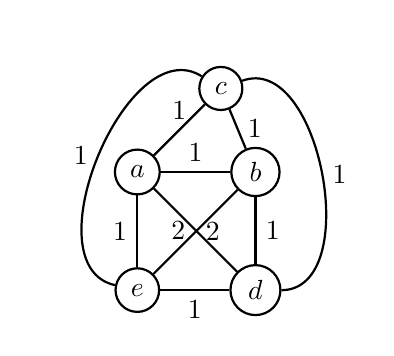
\begin{tikzpicture}[node distance={15mm}, thick, main/.style = {draw, circle}] 
            \node[main] (a) {$a$}; 
            \node[main] (b) [right of=a] {$b$}; 
            \node[main] (d) [below of=b] {$d$};
            \node[main] (e) [below of=a] {$e$};
            \node[main] (c) [above right of=a] {$c$}; 

            \draw (a) -- node[above] {1} (b); 
            \draw (a) -- node[above] {1} (c); 
            \draw (a) -- node[left] {1} (e);
            \draw (a) -- node[left] {2} (d);
            \draw (b) -- node[right] {1} (d);
            \draw (b) -- node[right] {1} (c);
            \draw (b) -- node[right] {2} (e);
            \draw (e) -- node[below] {1} (d);
            \draw (c) edge[bend right = 100] node[left] {1} (e);
            \draw (c) edge[bend left = 100] node[right] {1} (d);
            
            
\end{tikzpicture}\newline\newline
We can build the following MST $T^*$:\newline\newline
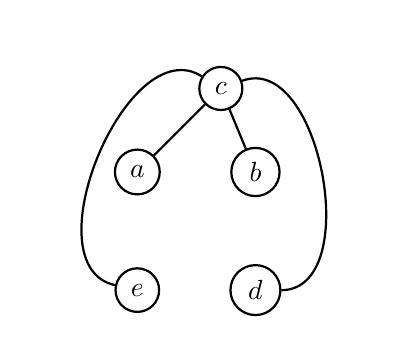
\begin{tikzpicture}[node distance={15mm}, thick, main/.style = {draw, circle}] 
            \node[main] (a) {$a$}; 
            \node[main] (b) [right of=a] {$b$}; 
            \node[main] (d) [below of=b] {$d$};
            \node[main] (e) [below of=a] {$e$};
            \node[main] (c) [above right of=a] {$c$}; 

            \draw (a) -- (c); 
            \draw (b) -- (c);
            \draw (c) edge[bend right = 100] (e);
            \draw (c) edge[bend left = 100]  (d);
\end{tikzpicture}\newline\newline
The odd-degree vertices are $a, b, e, d$. Then, a possible min-weight perfect matching $M^*$ is the following:\newline\newline
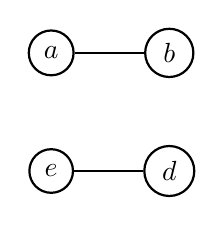
\begin{tikzpicture}[node distance={15mm}, thick, main/.style = {draw, circle}] 
            \node[main] (a) {$a$}; 
            \node[main] (b) [right of=a] {$b$}; 
            \node[main] (d) [below of=b] {$d$};
            \node[main] (e) [below of=a] {$e$};
            

            \draw (a) -- (b); 
            \draw (e) -- (d);
\end{tikzpicture}\newline\newline
Finally, the graph $G^* = (V, E^*) \cup M^*$ becomes the following:\newline\newline
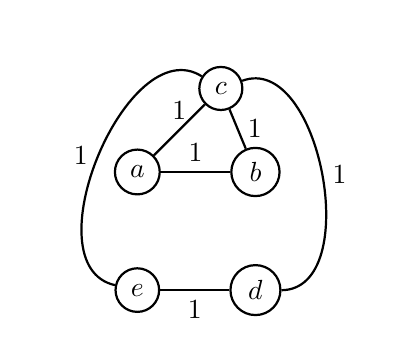
\begin{tikzpicture}[node distance={15mm}, thick, main/.style = {draw, circle}] 
            \node[main] (a) {$a$}; 
            \node[main] (b) [right of=a] {$b$}; 
            \node[main] (d) [below of=b] {$d$};
            \node[main] (e) [below of=a] {$e$};
            \node[main] (c) [above right of=a] {$c$}; 

            \draw (a) -- node[above] {1} (b); 
            \draw (a) -- node[above] {1} (c); 
            \draw (b) -- node[right] {1} (c);
            \draw (e) -- node[below] {1} (d);
            \draw (c) edge[bend right = 100] node[left] {1} (e);
            \draw (c) edge[bend left = 100] node[right] {1} (d);
            
            
\end{tikzpicture}\newline\newline
An Eulerian cycle computed on this grapg can be: $c, d, e, c, b, a, c$. We can find shortcuts as we did for \textit{APPROX\_METRIC\_TSP} and the final Tour $H$ becomes: $c, d, e, b, a, c$

\subsection{Analysis}
\begin{enumerate}
    \item $w(H) \leq w(T^*) + w(M^*)$ due to triangle inequality
    \item $w(T^*) \leq w(H^*)$
\end{enumerate}
We want to prove that $w(H) \leq \frac{3}{2}w(H^*)$\newline\newline
It can be proved that $w(M^*) \leq \frac{1}{2}w(H^*)$ \footnote{see lecture notes}. Then, putting all together:
\[w(H) \leq w(H^*) + \frac{w(H^*)}{2} = \frac{3}{2} w(H^*)\]

